Prolog: Programming in Logic\\
Prolog-Programme sind im Wesentlichen Hornformeln, bei denen alle Variablen allquantisiert sind. Jede Klausel ist dabei eine Zeile eines Prolog-Programmes.

\cparagraph{Beispiel}$ $
\begin{lstlisting}[language=Prolog]
katze(reni).
haustier(X):-katze(X).
\end{lstlisting}
Dieses Prolog-Programm stellt die Hornformel $katze(reni) \wedge \forall x \, (katze(x) \to haustier(x))$ dar.\\
Anfrage an den Prolog-Interpreter:
\begin{lstlisting}[language=Prolog]
?-haustier(reni).
true.
\end{lstlisting}

\section{Syntax}
Prädikat: Wort in Kleinbuchstaben.\\
Konstante: Wort in Kleinbuchstaben.\\
(Bestimmung ob Prädikat oder Konstante erfolgt über die Position des Wortes: Konstanten treten immer in der Klammer von Prädikaten auf)\\
Variable: Wort, das mit einem Großbuchstaben beginnt.\\
„ $\leftarrow$ “: „ \lstinline$:-$ “ (wird impliziert von).\\
„ $\wedge$ “: „ \lstinline$,$ “.\\
Jede Klausel wird mit „ \lstinline$.$ “ abgeschlossen. Alle Klauseln sind implizit mit $\wedge$ verknüpft.

\subsection*{$\vee$-Verknüpfung}
\lecdate{03.04.2017}
Die Formel $A\vee B \to C$ ist wegen $A\vee B \to C \equiv (\neg A \wedge \neg B ) \vee C$ keine Hornklausel. Da jedoch $(\neg A \wedge \neg B ) \vee C \equiv (\neg A \vee C) \wedge (\neg B \vee C) \equiv (A\to C) \wedge (B \to C)$, lässt sich $A \vee B \to C$ als Hornformel darstellen.\\
Daher gibt es in Prolog den $\vee$-Operator „ \lstinline$;$ “.
\cparagraph{Beispiel} Die Formel $\forall x \; (katze(x) \vee kater(x) \to tier(x) )$ kann in Prolog als Hornformel dargestellt werden durch:
\begin{lstlisting}[language=Prolog]
tier(X) :- katze(X).
tier(X) :- kater(X).
\end{lstlisting}
Die skann mit dem $\vee$-Operator abgekürzt werden durch \lstinline$tier(X) :- katze(X) ; kater(X).$\\
Die Variable \lstinline$X$ ist implizit allquantisiert (alle Variablen sind in Prolog allquantifiziert).

\subsection{Unterschied zwischen Prolog und imperativen Programmiersprachen}
Eine Variable kann sowohl Eingabe als auch Ausgabe sein. In einer imperativen Programmiersprache lässt sich nachbilden, dass eine Variable entweder Eingabe oder Ausgabe ist.\\
Prolog:
\begin{lstlisting}[language=Prolog]
katze(reni).
katze(mimi).
kater(momo).
tier(X) :- katze(X) ; kater(X).
\end{lstlisting}
Nachbildung in Java:
\begin{lstlisting}[language=Java]
Boolean katze(String x) {
	return x.equals("reni") || x.equals("mimi");
}

Boolean katze(String x) {
	return x.equals("momo");
}

Boolean tier(String x) {
	return katze(x) || kater(x);
}
\end{lstlisting}
Damit können wir die Anfrage für \lstinline$tier("momo")$ stellen, aber keine Anfrage \lstinline$tier(X)$ wie in Prolog, die alle \lstinline$X$ mit \lstinline$tier(X)$ wahr liefert.

\subsection{Existenzquantoren in Prolog durch Skolemisierung}
In Prolog sind alle vorkommenden Variablen allquantisiert. Daher können existenzquantisierte Variablen nicht unmittelbar dargestellt werden. Existenzquantoren können jedoch durch Skolemisierung eliminiert werden. Einfacher Spezialfall: Einführung einer Skolemkonstante.\\
Eine Formel der Form
$$\exists x\; P(X)$$
kann erfüllbarkeitsäquivalent umgeformt werden zu
$$P(a)$$
wobei $a$ eine noch nicht verwendete Konstante ist (Skolemkonstante).\\
So wird die Abfrage $\exists x\; katze(X)$ beispielsweise durch \lstinline$katze(reni)$ umgesetzt.

\subsection{Weiter Syntax}
\begin{tabular}{L{.3} L{.7}}
\lstinline$test(X,_)$ & \lstinline$_$ ist anonyme Variable / Platzhalter, falls Variable im Kontext nicht relevant ist.\\
\lstinline$not(X=Y)$ oder \lstinline$X\=Y$ & Prüfung, ob \lstinline$X$ ungleich (im Sinne von „nicht unifizierbar“) \lstinline$Y$.\\
\lstinline$\+ (...)$ & Aussage \lstinline$...$ wird negiert (ähnlich wie die Prüfung \lstinline$not(...)$).
\end{tabular}

\section{Auswertstrategie in Prolog}
Die Struktur  eines Prolog-Programmes lässt sich durch einen Und-Oder-Baum darstellen:\bigskip\\
Und-Verknüpfung: \lstinline$a(X) :- b(X) , c(X) , d(X).$\\
\begin{tabular}{L{.3} L{.7}}
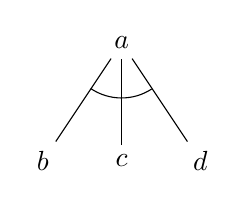
\begin{tikzpicture}
\node (v2) at (-0.5,1) {$a$};
\node (v1) at (-1.5,-0.5) {$b$};
\node (v4) at (-0.5,-0.5) {$c$};
\node (v3) at (0.5,-0.5) {$d$};
\draw (v1) -- (v2) -- (v3);
\draw (v4) -- (v2);
\def\wa{-57};\def\wb{-124}\def\rd{.7cm};
\draw[shift=(\wa : \rd)] (-.5,1) arc (\wa:\wb:\rd);
\end{tikzpicture} & \mpb[.6]
Für die Anfrage \lstinline$a(X)$ werden die Zeilziele \lstinline$b(X)$, \lstinline$c(X)$, \lstinline$d(X)$ erzeugt, die alle wahr sein müssen.
\mpe
\end{tabular}\\
Oder-Verknüfung: \lstinline$a(X) :- b(X) ; c(X) ; d(X).$\\
\begin{tabular}{L{.3} L{.7}}
\begin{tikzpicture}
\node (v2) at (-0.5,1) {$a$};
\node (v1) at (-1.5,-0.5) {$b$};
\node (v4) at (-0.5,-0.5) {$c$};
\node (v3) at (0.5,-0.5) {$d$};
\draw (v1) -- (v2) -- (v3);
\draw (v4) -- (v2);
\end{tikzpicture} & \mpb[.6]
Hier muss eines der Teilziele wahr sein.
\mpe
\end{tabular}

\cparagraph{Beispiel} Programm von oben:
\begin{center}
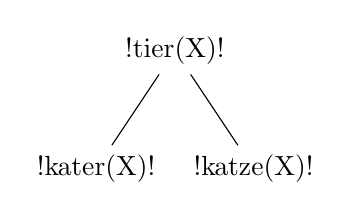
\begin{tikzpicture}
\node (v2) at (-0.5,1) {\lstinline!tier(X)!};
\node (v1) at (-1.5,-0.5) {\lstinline!kater(X)!};
\node (v3) at (0.5,-0.5) {\lstinline!katze(X)!};
\draw (v1) -- (v2) -- (v3);
\end{tikzpicture}
\end{center}
Bei der Anfrage \lstinline$tier(X)$ wird die Variable \lstinline$X$ ersetzt durch die Konstante \lstinline$reni$ und die Variablen auf tieferen Ebenen werden entsprechend ersetzt.\\
Schreibweise: \lstinline$X/reni$ (\lstinline$X$ wird unifiziert mit \lstinline$reni$)
\begin{center}
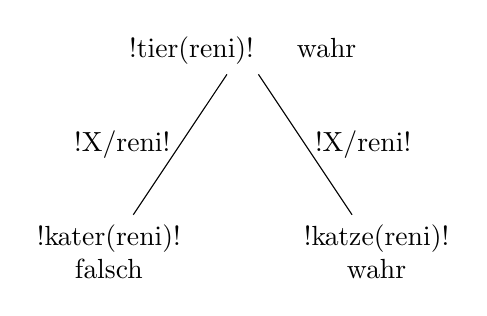
\begin{tikzpicture}[scale=1.7]
\node (v2) at (-0.5,1) {\lstinline!tier(reni)! ~~ wahr};
\node[align=center] (v1) at (-1.5,-0.5) {\lstinline!kater(reni)!\\ falsch};
\node[align=center] (v3) at (0.5,-0.5) {\lstinline!katze(reni)!\\ wahr};
\draw (v1) -- node[left]{\lstinline!X/reni!} (v2) -- node[right]{\lstinline!X/reni!} (v3);
\end{tikzpicture}
\end{center}
Allgemein kann ein Und-Oder-Baum aus beliebig vielen Und- oder Oder-Verknüpfungen bestehen.\\
Dieser Baum muss systematisch durchsucht werden, um einen Wahrheitswert für die Wurzel zu bestimmen.\\
Mögliche Strategien: Tiefensuche, Breitensuche.
\subsection{Tiefensuche}
Problem bei der Tiefensuche:
\cparagraph{Beispiel} $ $
\begin{lstlisting}[language=Prolog]
zug(X,Y) :- zug (Y,X).
zug(1,2).
\end{lstlisting}
Anfrage \lstinline$zug(2,1)$:
\begin{center}
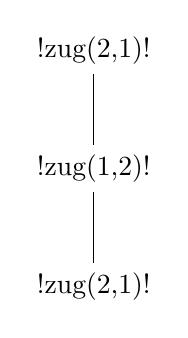
\begin{tikzpicture}
\node (v1) at (0,3.5) {\lstinline!zug(2,1)!};
\node (v2) at (0,2) {\lstinline!zug(1,2)!};
\node (v3) at (0,0.5) {\lstinline!zug(2,1)!};
\draw (v1) -- (v2) -- (v3);
\end{tikzpicture}
\end{center}
Der Und-Oder-Baum ist unendlich und eine Tiefensuche, die den ersten Zweig (links) verfolgt, findet keine Lösung.\\
Das gleiche Problem tritt bei einer entsprechenden Implementierung in Java auf:
\begin{lstlisting}[language=Java]
Boolean zug(int x, int y) {
	return zug(y,x) || (x==1 && y==2);
}
\end{lstlisting}
\subsection{Breitensuche}
Die Breitensuche würde hier eine Lösung finden:
\begin{center}
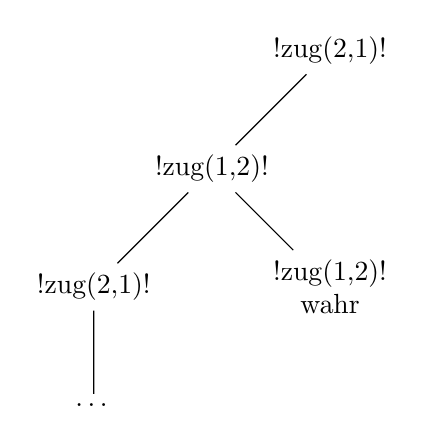
\begin{tikzpicture}
\node (v0) at (0,1.5) {\lstinline!zug(2,1)!};
\node (v3) at (-1.5,0) {\lstinline!zug(1,2)!};
\node (v2) at (-3,-1.5) {\lstinline!zug(2,1)!};
\node [align=center] (v4) at (0,-1.5) {\lstinline!zug(1,2)!\\ wahr};
\node (v1) at (-3,-3) {…};
\draw (v1) -- (v2) -- (v3) -- (v0);
\draw (v3) -- (v4);
\end{tikzpicture}
\end{center}
Das heißt, die Breitensuche liefert eine Lösung, die Tiefensuche unter Umständen nicht.\bigskip\\
Lösung: Die Abbruchbedingung der Rekursion muss die erste Klausel sein damit die Rekursion nicht endlos läuft bzw. die Tiefensuche die Abzweigung nimmt, die zu einer Lösung führt:
\begin{lstlisting}[language=Prolog]
zug(1,2).
zug(X,Y) :- zug(Y,X).
\end{lstlisting}

\subsection{Unifizierbarkeit}
\lecdate{10.04.2017}
\cparagraph{Definition} Zwei Atome $P,Q$ heißen \emph{unifizierbar}, wenn es eine Ersetzung der in $P,Q$ vorkommenden Variablen gibt, so dass damit $P\equiv Q$.

\cparagraph{Beispiel} Mit $a,\; b,\; c$ … Konstanten, $x,\; y ,\; z$ … Variablen.
\begin{itemize}
\item $P(x,a),\; P(a,a)$ sind unifizierbar durch $x/a$.
\item $Q(a,x,y),\; Q(z,b,c)$ sind unifizierbar durch $z/a,\; x/b,\; y/c$.
\item $P(x,x)\; P(a,b)$ sind nicht unifizierbar.
\end{itemize}

$\to$ Auswertstrategie von Prolog:\\
Für ein Ziel $P$ wird das Prolog-Programm von oben nach unten durchsucht, bis eine linke Seite einer Klausel (das, was hinter der Implikation steht bzw. in Prolog vor \lstinline$:-$) mit $P$ unifiziert. Indem die rechte Seite der Klausel ebenso ersetzt wird, werden neue Teilziele erzeugt.

\cparagraph{Beispiel} $ $
\begin{lstlisting}[language=Prolog]
zug(1,2).							% (1)
zug(X,Y):- zug(Y,X).	% (2)
\end{lstlisting}
Für die Anfrage \lstinline$zug(2,1)$ wird folgender Suchbaum erzeugt:
\begin{center}
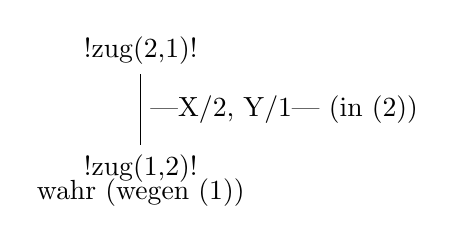
\begin{tikzpicture}
\node (v1) at (0,3.5) {\lstinline!zug(2,1)!};
\node (v2) at (0,2) {\lstinline!zug(1,2)!};
\node[below] at (v2) {wahr (wegen (1))};
\draw (v1) -- node[right, pos=.5]{\lstinline|X/2, Y/1| (in (2))} (v2);
\end{tikzpicture}
\end{center}
Wenn beispielsweise 
\begin{lstlisting}[language=Prolog]
q(X,Y):- (a,b).
r(Y):- (b).
p(X):- q(X,Y) , r(Y).
\end{lstlisting}
dann:
\begin{center}
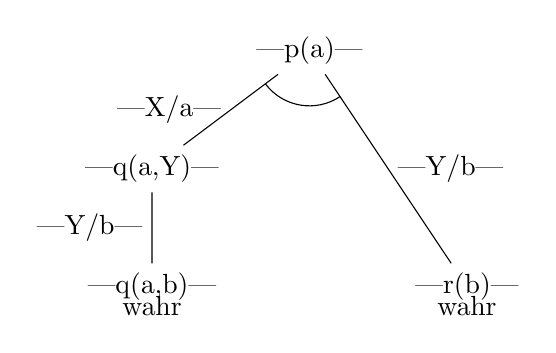
\begin{tikzpicture}
\node (v1) at (-1,2.5) {\lstinline|p(a)|};
\node (v2) at (-3,1) {\lstinline|q(a,Y)|};
\node (v3) at (-3,-0.5) {\lstinline|q(a,b)|};
\node (v4) at (1,-0.5) {\lstinline|r(b)|};
\node[below] at (v3) {wahr};
\node[below] at (v4) {wahr};
\draw (v1) -- node[left]{\lstinline|X/a|} (v2) -- node[left]{\lstinline|Y/b|} (v3);
\draw (v1) -- node[right]{\lstinline|Y/b|} (v4);
\def\wa{-56};\def\wb{-143}\def\rd{.7cm};
\draw[shift=(\wa : \rd)] (-1,2.5) arc (\wa:\wb:\rd); %%%TODO
\end{tikzpicture}
\end{center}

\subsection{Backtracking}
Wenn das neue Teilziel \lstinline|false| liefert, wird ein Backtracking ausgeführt und eine andere Alternative gesucht.

\cparagraph{Beispiel}$ $
\begin{lstlisting}[language=Prolog]
q(X):- p(X).	% (1)
q(X):- r(X).	% (2)
p(a).
r(b).
\end{lstlisting}
Anfrage: \lstinline$q(b)$\\
Suchbaum:
\begin{center}
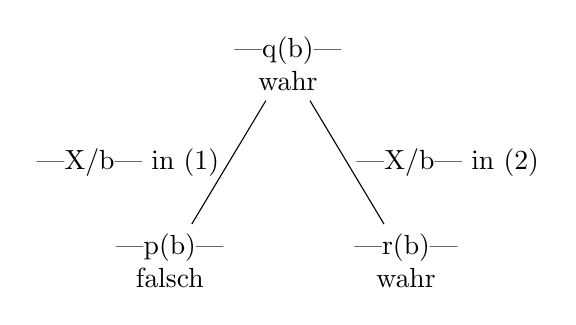
\begin{tikzpicture}
\node [align=center] (v1) at (-1,2.5) {\lstinline|q(b)|\\wahr};
\node [align=center] (v2) at (-2.5,0) {\lstinline|p(b)|\\falsch};
\node [align=center] (v3) at (.5,0) {\lstinline|r(b)|\\wahr};
\draw (v1) -- node[left,pos=.5]{\lstinline|X/b| in (1)} (v2);
\draw (v1) -- node[right, pos=.5]{\lstinline|X/b| in (2)} (v3);
\end{tikzpicture}
\end{center}
Bei einer Und-Verknüpfung im Suchbaum wird zuerst der linke Teilbaum durchsucht, dann die rechten Teilbäume, wobei jeweils die gleichen Ersetzungen von Variablen vorgenommen werden.
\cparagraph{Beispiel} $ $
\begin{lstlisting}[language=Prolog]
p(X):- q(X), r(X).
\end{lstlisting}
Anfrage: \lstinline$p(X)$
Suchbaum:
\begin{center}
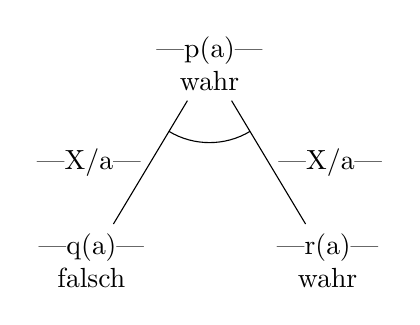
\begin{tikzpicture}
\node [align=center] (v1) at (-1,2.5) {\lstinline|p(a)|\\wahr};
\node [align=center] (v2) at (-2.5,0) {\lstinline|q(a)|\\falsch};
\node [align=center] (v3) at (.5,0) {\lstinline|r(a)|\\wahr};
\draw (v1) -- node[left,pos=.5]{\lstinline|X/a|} (v2);
\draw (v1) -- node[right, pos=.5]{\lstinline|X/a|} (v3);
\def\wa{-59};\def\wb{-121}\def\rd{1cm};
\draw[shift=(\wa : \rd)] (-1,2.5) arc (\wa:\wb:\rd);
\end{tikzpicture}
\end{center}
Die Auswertstrategie von oben nach unten lässt sich nutzen, um ein \lstinline$if-else$ zu implementieren.
\cparagraph{Beispiel}$ $
\begin{lstlisting}[language=Prolog]
strassenzustand(regen,nass).
strassenzustand(X,trocken).
\end{lstlisting}
Anfrage 1: 
\begin{center}
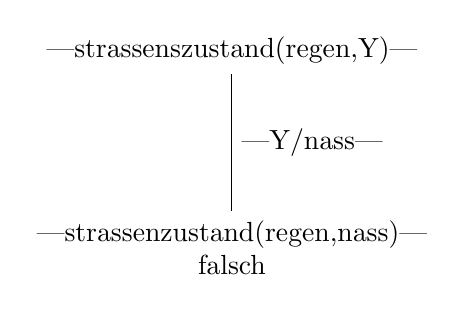
\begin{tikzpicture}
\node [align=center] (v1) at (-1,2.5) {\lstinline|strassenszustand(regen,Y)|};
\node [align=center] (v2) at (-1,0) {\lstinline|strassenzustand(regen,nass)|\\ falsch};
\draw (v1) -- node[right,pos=.5]{\lstinline|Y/nass|} (v2);
\end{tikzpicture}
\end{center}
Anfrage 2:
\begin{center}
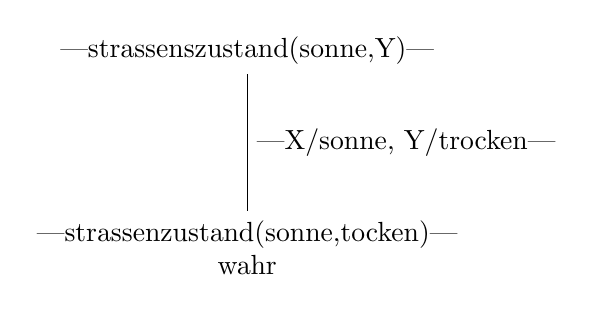
\begin{tikzpicture}
\node [align=center] (v1) at (-1,2.5) {\lstinline|strassenszustand(sonne,Y)|};
\node [align=center] (v2) at (-1,0) {\lstinline|strassenzustand(sonne,tocken)|\\ wahr};
\draw (v1) -- node[right,pos=.5]{\lstinline|X/sonne, Y/trocken|} (v2);
\end{tikzpicture}
\end{center}
Um zu verhindern, dass auch \lstinline$strassenzustand(regen, trocken)$ zu wahr auswertet, kann die zweite Zeile zu \lstinline$strassenzustand(X,trocken):- X \== regen$ geändert werden.

\section{Darstellung von Relationen in Prolog}
Eine endliche Relation kann durch Aufzählung dargestellt werden. Reflexive, transitive und symmetrische Relationen werden durch entsprechende Regeln dargestellt.
\begin{itemize}
\item Wenn \lstinline$p(X,Y)$ eine Relation ist, kann deren symmetrische Hülle dargestellt werden durch \lstinline$q(X,Y):- p(X,Y); p(Y,X).$
\item Die reflexive Hülle von \lstinline$p$ wird erzeugt, indem die Regel \lstinline$p(X,X)$ hinzugefügt wird.
\item Naiver Versuch Transitivität:
\begin{lstlisting}[language=Prolog]
p(X,Y).
q(X,Z):- p(X,Z); p(X,Y), p(Y,Z).\\
% Achtung: Funktioniert nur für Wege der Länge 2!
\end{lstlisting}
$\to$ Berechnung der transitiven Hülle einer Relation.
\end{itemize}

\subsection{Transitive Hülle}
Sei \lstinline$weg/2$ eine binäre Relation, von der wir die transitive Hülle  berechnen wollen. Es gilt:\\
Es gibt einen Weg von $X$ nach $Y$ genau dann wenn:
\begin{itemize}
\item $X=Y$ oder
\item es gibt einen Knoten $z$ und einen Weg von $X$ nach $Z$ und von $Z$ nach $Y$.
\end{itemize}
Wir müssen daher die reflexive und transitive Hülle von \lstinline$weg$ berechnen.\\
Als Formel:
\begin{align*}
&\forall X\; weg(X,X) \wedge\\
&\forall X \;\forall Y \; ((\exists Z\; weg(X,Z) \wedge weg(Z,Y)) \to weg(X,Y))
\end{align*}
Um den Existenzquantor zu beseitigen formen wir die zweite Klausel um:
\begin{align*}
&\forall X\; \forall Y\; (\forall Z\; \neg weg(X,Z) \vee \neg weg(Z,Y) \vee weg(X,Y))\\
\equiv & \forall X\; \forall Y\; \forall Z\;(\neg weg(X,Z) \vee \neg weg(Z,Y) \vee weg(X,Y))\\
\equiv& \forall X\; \forall Y\; \forall Z\;( weg(X,Z) \wedge weg(Z,Y) \to weg(X,Y))
\end{align*}
In Prolog bspw.:
\begin{lstlisting}[language=Prolog]
weg(a,b).
weg(b,c).
weg(c,d).
weg(X,X).
weg(X,Y):- weg(X,Z), weg(Z,Y).
\end{lstlisting}
Anfrage 1:
\begin{center}
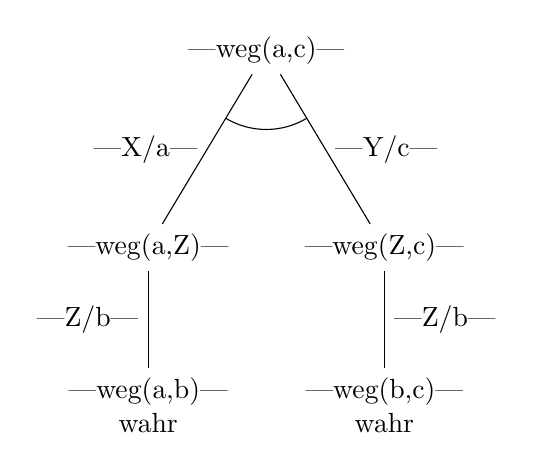
\begin{tikzpicture}
\node [align=center] (v1) at (-1,2.5) {\lstinline|weg(a,c)|};
\node [align=center] (v2) at (-2.5,0) {\lstinline|weg(a,Z)|};
\node [align=center] (v3) at (-2.5,-2) {\lstinline|weg(a,b)|\\wahr};
\node [align=center] (v4) at (.5,0) {\lstinline|weg(Z,c)|};
\node [align=center] (v5) at (.5,-2) {\lstinline|weg(b,c)|\\wahr};
\draw (v1) -- node[left,pos=.5]{\lstinline|X/a|} (v2);
\draw (v2) -- node[left, pos=.5]{\lstinline|Z/b|} (v3);
\draw (v1) -- node[right,pos=.5]{\lstinline|Y/c|} (v4);
\draw (v4) -- node[right, pos=.5]{\lstinline|Z/b|} (v5);
\def\wa{-59};\def\wb{-121}\def\rd{1cm};
\draw[shift=(\wa : \rd)] (-1,2.5) arc (\wa:\wb:\rd);
\end{tikzpicture}
\end{center}
Anfrage 2:
\begin{center}
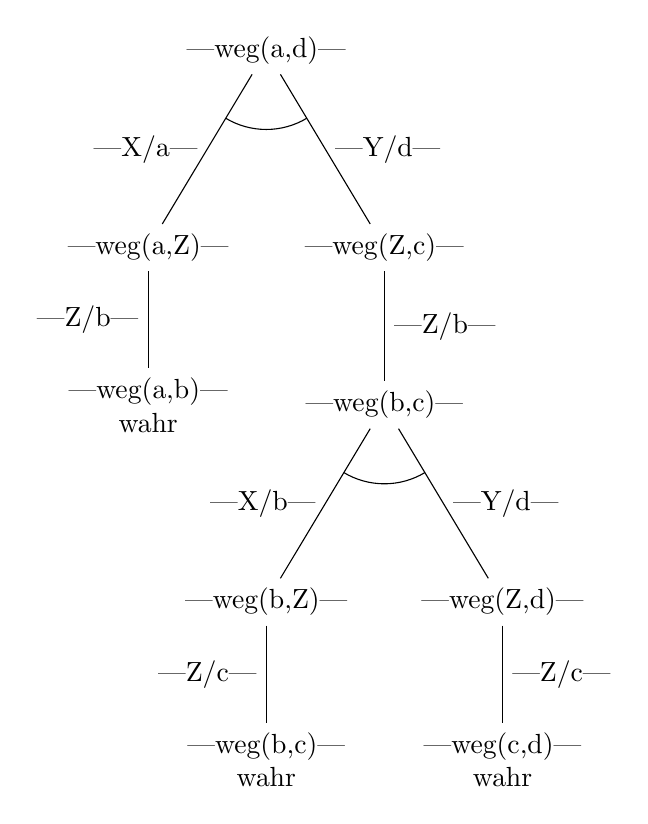
\begin{tikzpicture}
\node [align=center] (v1) at (-1,2.5) {\lstinline|weg(a,d)|};
\node [align=center] (v2) at (-2.5,0) {\lstinline|weg(a,Z)|};
\node [align=center] (v3) at (-2.5,-2) {\lstinline|weg(a,b)|\\wahr};
\node [align=center] (v4) at (.5,0) {\lstinline|weg(Z,c)|};
\node [align=center] (v5) at (.5,-2) {\lstinline|weg(b,c)|};
\node [align=center] (v6) at (-1,-4.5) {\lstinline|weg(b,Z)|};
\node [align=center] (v7) at (-1,-6.5) {\lstinline|weg(b,c)|\\wahr};
\node [align=center] (v8) at (2,-4.5) {\lstinline|weg(Z,d)|};
\node [align=center] (v9) at (2,-6.5) {\lstinline|weg(c,d)|\\wahr};
\draw (v1) -- node[left,pos=.5]{\lstinline|X/a|} (v2);
\draw (v2) -- node[left, pos=.5]{\lstinline|Z/b|} (v3);
\draw (v1) -- node[right,pos=.5]{\lstinline|Y/d|} (v4);
\draw (v4) -- node[right, pos=.5]{\lstinline|Z/b|} (v5);
\draw (v5) -- node[left, pos=.5]{\lstinline|X/b|} (v6);
\draw (v6) -- node[left, pos=.5]{\lstinline|Z/c|} (v7);
\draw (v5) -- node[right, pos=.5]{\lstinline|Y/d|} (v8);
\draw (v8) -- node[right, pos=.5]{\lstinline|Z/c|} (v9);
\def\wa{-59};\def\wb{-121}\def\rd{1cm};
\draw[shift=(\wa : \rd)] (-1,2.5) arc (\wa:\wb:\rd);
\draw[shift=(\wa : \rd)] (.5,-2) arc (\wa:\wb:\rd);
\end{tikzpicture}
\end{center}

\section{Computeralgebra}
\lecdate{24.04.2017}
\subsection{Arithmetik in Prolog}
Arithmetische Ausdrücke werden mit dem Operator \lstinline$is$ ausgewertet. Dabei muss die rechte Seite instantiiert sein.
\cparagraph{Beispiel}$ $
\begin{lstlisting}[language=Prolog]
?- X is 3+4.
X=7.
?- 10 is 3+4.
false.
?- 2 is 1+X
Fehler!!!
f(X,Y):- Y=3*X+1	% Falsch! = ist Unifikationsoperator, keine Funktionszuweisung
f(1,Y).
Y=3*1+1.
\end{lstlisting}

\subsection{Vergleichsoperatoren}
\begin{tabular}{c l l}
Operator & Bedeutung & Beispiel\\\hline
\lstinline$==$ & identisch & \lstinline$p(X) == p(X)$\\
\lstinline$\==$ & nicht identisch & \lstinline$p(X) \== p(Y)$\\
\lstinline$=$ & unifizierbar & \lstinline$p(X) = p(Y)$\\
\lstinline$\=$ & nicht unifizierbar & \lstinline$p(X) \= q(X)$\\
\lstinline$=:=$ & arithmetisch gleich & \lstinline$2 =:= 1+1$\\
\lstinline$=\=$ & arithmetisch ungleich & \lstinline$3 =\= 1+1$
\end{tabular}\\
In Prädikaten können Operatorsymbole wie $+, -, *, /, \hat{\,}$ verwendet werden, um arithmetische Ausdrücke zu zerlegen. Prolog berücksichtigt dabei die Priorität der Operatoren.
\cparagraph{Beispiel}$ $
\begin{lstlisting}[language=Prolog]
?- x + 3*y + x*2 = A + B + C.
A=x, B=3*y, C=x*2.
?- 2*x + 3*y = A + B * C.
A=2*x, B=3, C=y
?- 2*x + y + z = A + B % nicht eindeutig!
\end{lstlisting}

\subsection{Anwendung: Symbolisches Differenzieren}
Ziel: Wir wollen ein Prädikat \lstinline$diff/3$ (3-Stelliger Operator) definieren, mit dem Polynome symbolisch differenziert werden können.
\cparagraph{Beispiel} $ $
\begin{lstlisting}[language=Prolog]
diff(3*x^2+5x-2 , x , D).
D = 6*x+5.
\end{lstlisting}
\begin{lstlisting}[language=Prolog]
d(X,X,1).
d(C,X,0) :- atomic(C), C\==X.

?- d(x,x,D).
D = 1.
?- d(c,x,D).
D = 0.
?- d(x+y, x+y, D).
D = 1.

% weitere Ableitungsregel (Ableitung negativer Funktion):
d(-F,X,-DF) :- d(F,X,DF).

?- d(-x,x,D).
D = -1.

% weitere Ableitungsregel (Ableitung mit führender Konstante):
d(C*F,X,C*DF) :- d(C,X,0), d(F,X,DF).

?- d(3*x,x,D).
D = 3*1.

% weitere Ableitungsregel (Kettenregel):
d(F+G,X,DF+DG) :- d(F,X,DF), d(G,X,DG).
d(F-G,X,DF-DG) :- d(F,X,DF), d(G,X,DG).

?- d(3*x+5,x,D).
D = 3*1+0.

% weiter Ableitungsregel (einfache Ableitung): 
d(F^N,X,N*F^M):- number(N), M is N-1, d(F,X,DF).
\end{lstlisting}

\subsection{Vereinfachen von arithmetischen Ausdrücken}
Idee: Wir definieren elementare Vereinfachungsregeln und vereinfachen rekursiv.\\
Elementare Vereinfachungsregeln:
\begin{lstlisting}[language=Prolog]
s0(1*X,X).
s0(X*1,X).
s0(0+X,X).
s0(X+0,X).
%...
s0(X,X).	% Lösung zu folgendem Problem
\end{lstlisting}
Problem: Wenn ein Term bereits vereinfacht ist, liefert \lstinline$s0 false$. Zum Beispiel \lstinline$s0(x,X)$.\\
Lösung: Regel \lstinline$s0(X,X).$ am Ende hinzufügen (wenn keine der Regeln greift, ist Term schon vereinfacht).\\
Um Ausdrücke zu vereinfachen, die aus mehreren Termen bestehen, wenden wir die Vereinfachung rekursiv auf jeden Term an und vereinfachen das Ergebnis. Zum Beispiel: Ausdruck $1*x+3*1+0$
\begin{center}
\begin{tikzpicture}
\node at (-3.5,2) {$\underset{A}{\underline{1*x+3*1}}+\underset{B}{\underline{0}}$};
\draw (-2.5,1.5) -- (-2,0.5) node[below]{$0$};
\draw (-4,1.5) -- (-5,0.5) node[below]{$\underset{A}{\underline{1*x}}+\underset{B}{\underline{3*1}}$};
\draw (-5.5,-0.5) -- (-6,-1.5) node[below]{$x$};
\draw (-4.5,-0.5) -- (-4,-1.5) node[below]{$3$};
\node [left] at (-7,0) {Ergebnis: $x+3$};
\node [align=right, left] at (-7,2) {Ergebnis: $x+3+0$\\Veireinfachen gibt: $x+3$};
\end{tikzpicture}
\end{center}






















